\section{Waves}
\footnotetext{Notes based on 3blue1brown/minutephysics \url{https://www.youtube.com/watch?v=MzRCDLre1b4}}

\newpage
See \ref{real-and-complex-vector-spaces}
\section{Adjoint, Unitary matrices, etc}\label{adjoint-and-unitary-matrices}
The \defn{conjugate transpose} or \defn{adjoint} or \defn{Hermitian conjugate} of a matrix is formed
by taking the transpose, and then replacing each element with its complex conjugate:
\begin{align*}
  U^\dag = \bar{U^T}.
\end{align*}
It is also written as $U^*$ or $U^H$.

A matrix $U$ is \defn{unitary} if $U^\dag U = I$.

\newpage
\section{The qubit}
\footnotetext{Notes based on Michael Nielsen - Quantum Computing for the Very Curious \url{https://quantum.country/qcvc}}

The state of a qubit is a unit vector in a two-dimensional complex vector space. The basis vectors
are written $\ket{0}$ and $\ket{1}$, so a qubit is
\begin{align*}
  \alpha\ket{0} + \beta\ket{1}
\end{align*}
where $\alpha, \beta \in \C$ with $|\alpha|^2 + |\beta|^2 = 1$.

What does the normalization constraint $|\alpha|^2 + |\beta|^2 = 1$ mean geometrically? If
$\alpha = 0$ then $\beta$ lies on the unit circle, and vice versa.

How can we visualize the possible values of a qubit?

Perhaps like this? This diagram illustrates that we pick two complex numbers, $\alpha$ and $\beta$,
and that they satisfy $|\alpha|^2 + |\beta^2| = 1$.\\
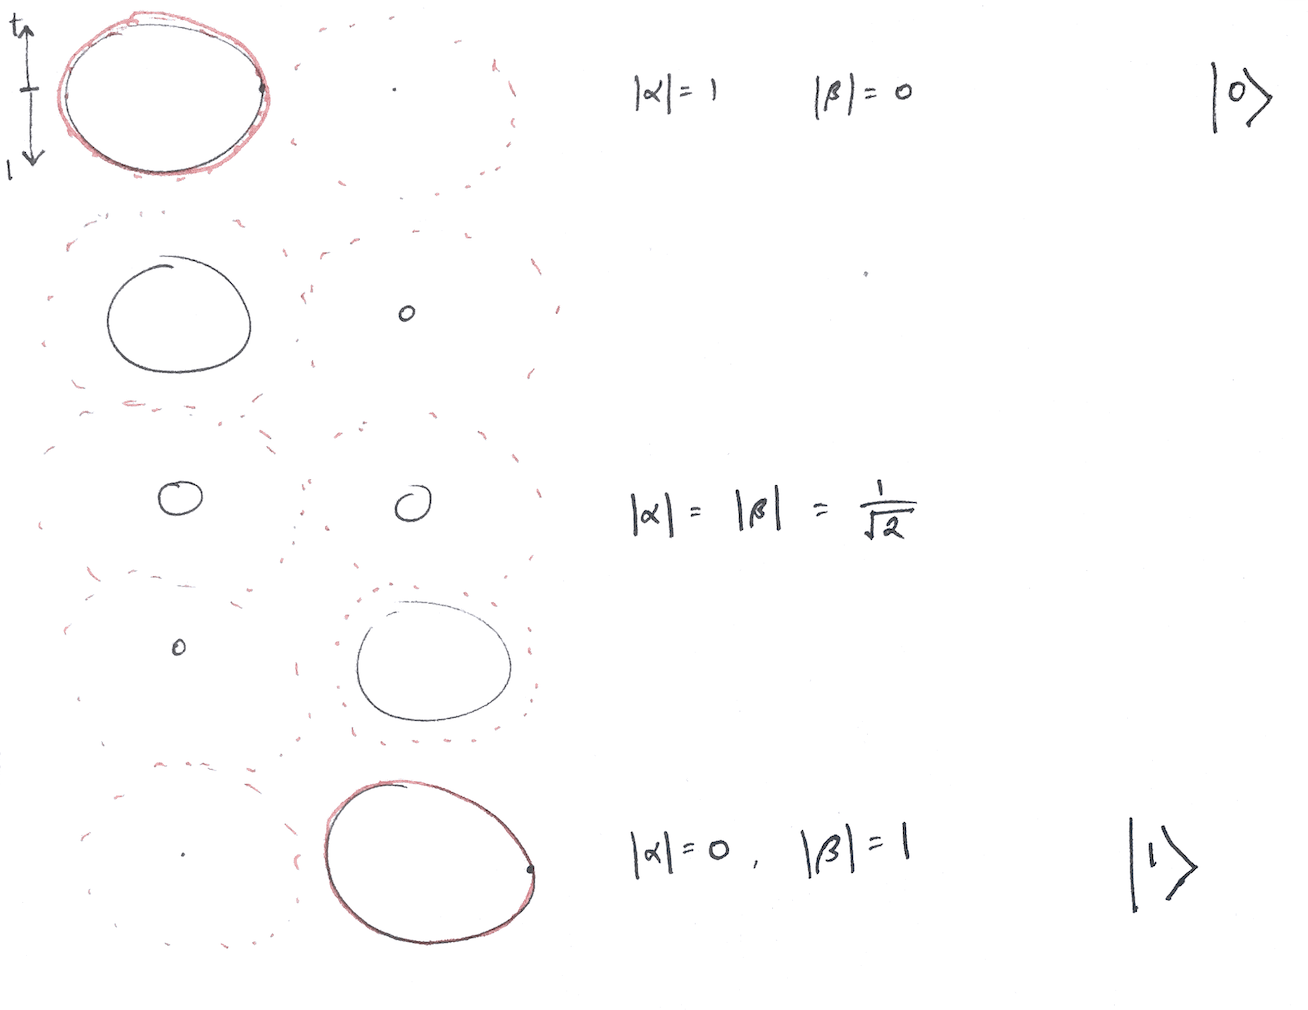
\includegraphics[width=200pt]{img/quantum-qubit-2.png}

Or like this? Visualize $(|\alpha|, |\beta|)$ as a point on the unit circle and place a clockface at
that point with two hands, representing the argument
of $\alpha$ and $\beta$.\\
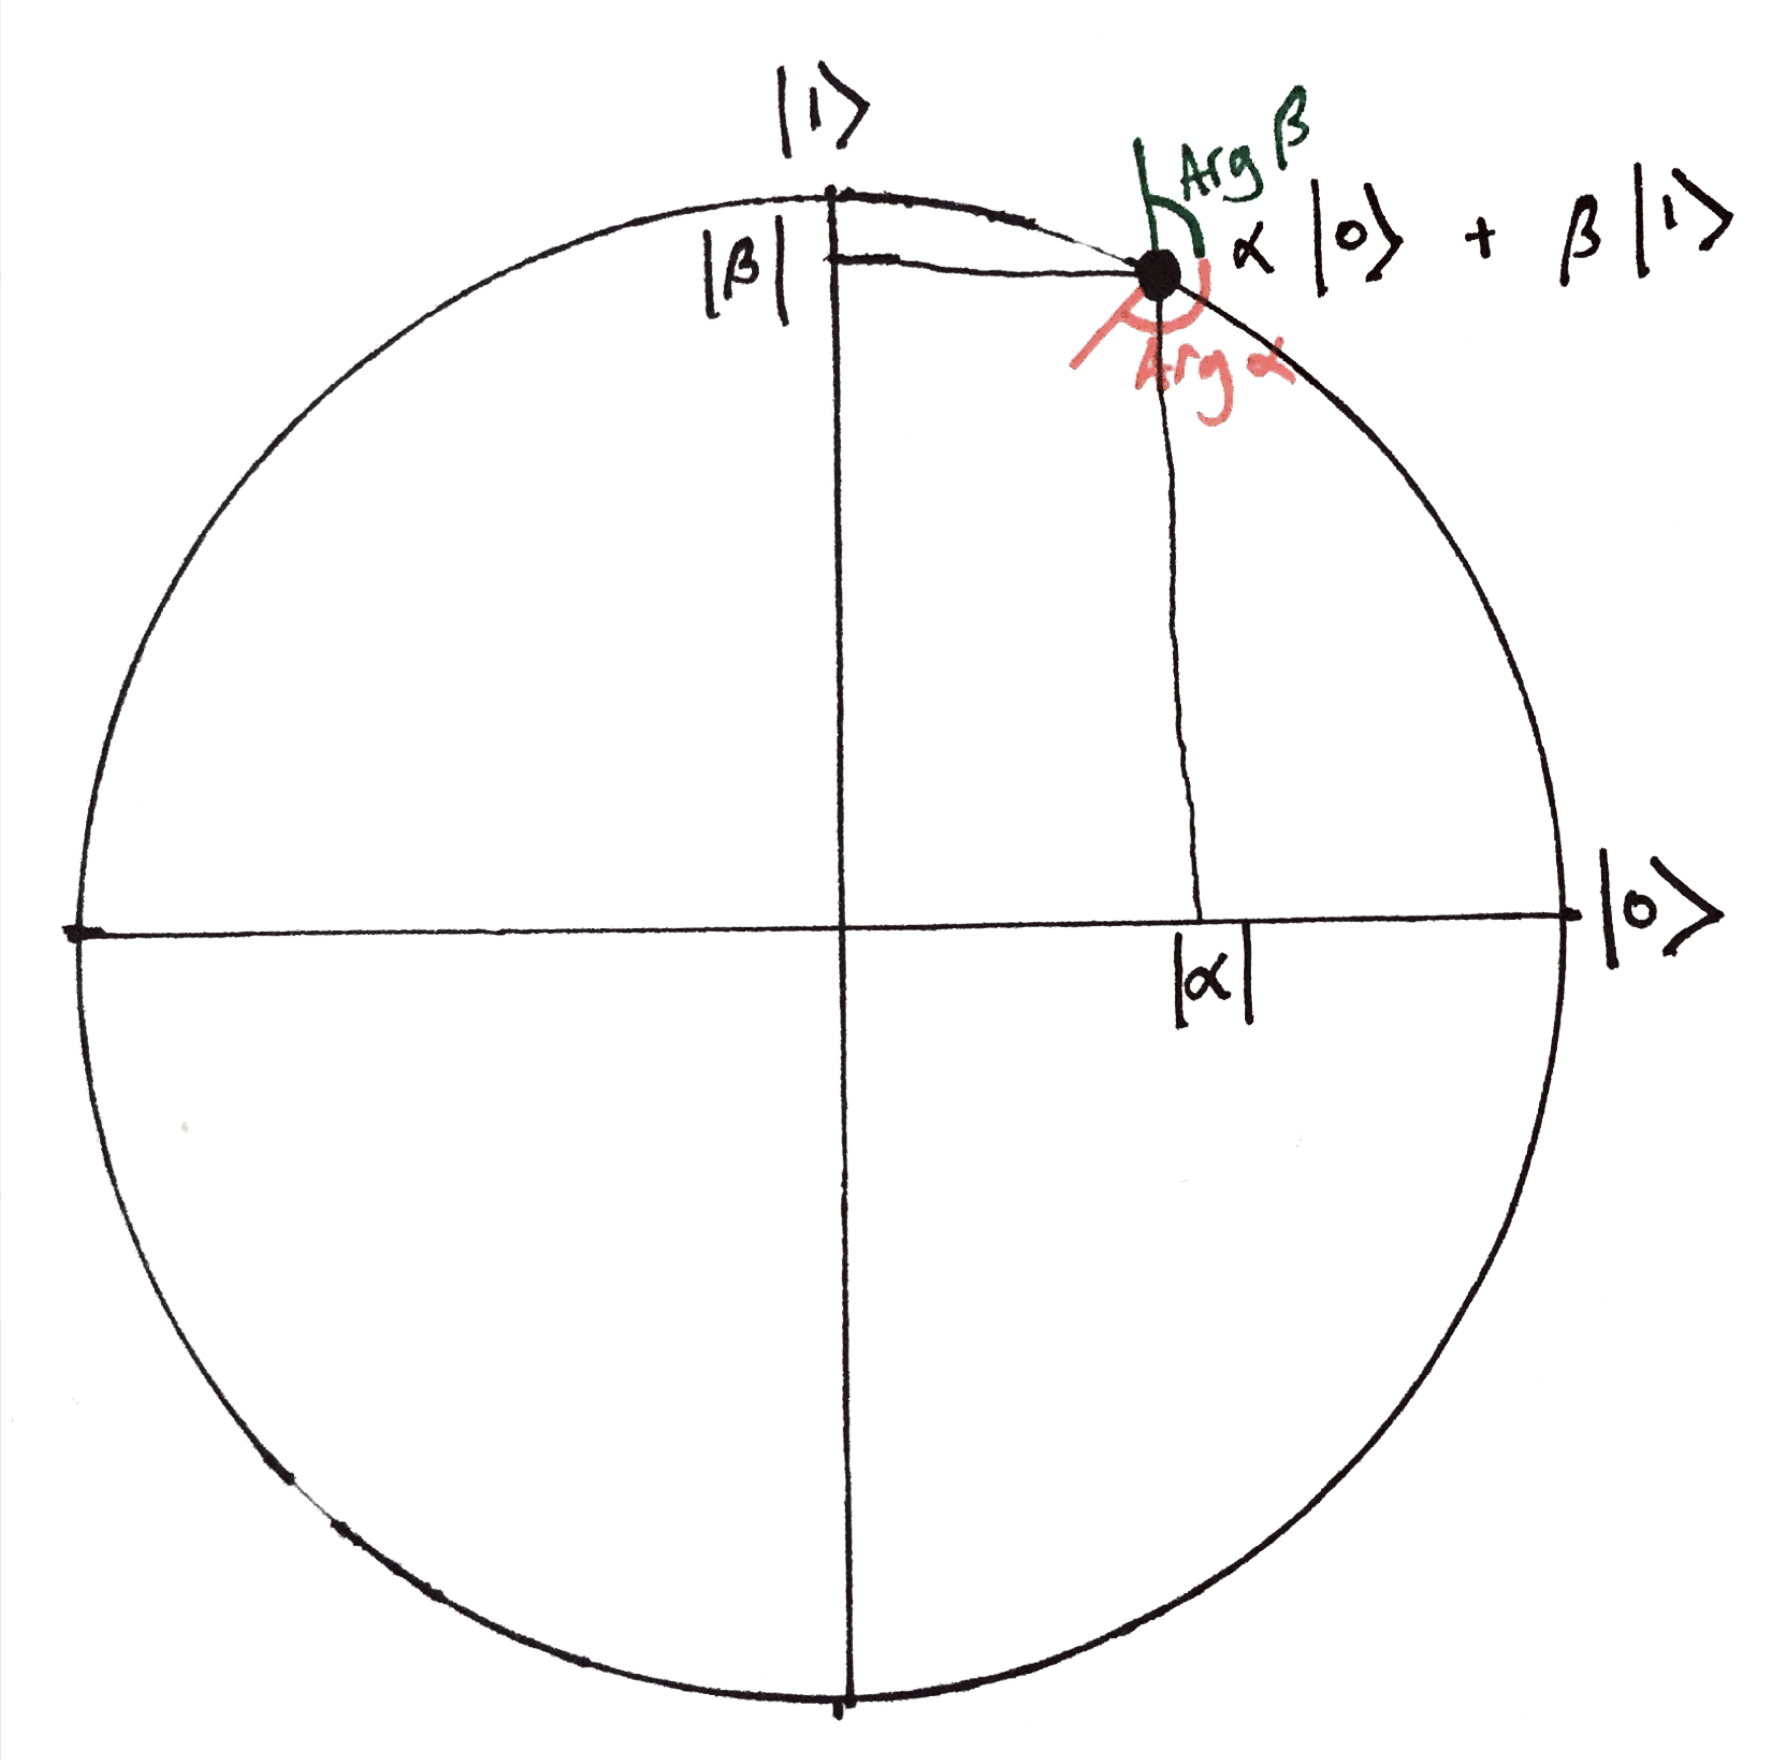
\includegraphics[width=200pt]{img/quantum-qubit.png}


\newpage


\newpage
\section{Quantum logic gates}

These are linear operators that act on a qubit state to produce a new qubit state. Therefore they
are $2 \times 2$ complex matrices. Since they unitary
\begin{enumerate}
\item {\bf Not}
  \begin{align*}
    X = \matMMxNN{0}{1}
    {1}{0}
  \end{align*}
\item {\bf Hadamard}
  \begin{align*}
    H = \frac{1}{\sqrt{2}}\matMMxNN{1}{1}
    {1}{-1}
  \end{align*}
\item {\bf $Y$}
  \begin{align*}
    Y = \matMMxNN{0}{-i}
                 {i}{0}
  \end{align*}
\item {\bf $Z$}
  \begin{align*}
    Z = \matMMxNN{1}{0}
                 {0}{-1}
  \end{align*}
\end{enumerate}

The not gate essentially swaps the two dimensions: the coefficient of $\ket{0}$ becomes the
coefficient of $\ket{1}$ and vice versa. So e.g.
\begin{align*}
  X\ket{0} &= \ket{1}\\
  X\ket{1} &= \ket{0},
\end{align*}
and by linearity
\begin{align*}
  X \(\alpha \ket{0} + \beta \ket{1}\) = \beta \ket{0} + \alpha \ket{1}
\end{align*}

Since they are real and symmetric, we have $X^\dag = X$ and $H^\dag = H$. And since
\begin{align*}
  X^2 &= I\\
  H^2 &= \frac{1}{2}\matMMxNN{2}{0}
        {0}{2} = I,
\end{align*}\
we have that $X$ and $H$ are unitary.


% \begin{align*}
%   H \ket{0} &= \frac{\ket{0}}{\sqrt{2}} + \frac{\ket{1}}{\sqrt{2}}\\
%   H \ket{1} &= \frac{\ket{0}}{\sqrt{2}} - \frac{\ket{1}}{\sqrt{2}}
% \end{align*}
